\clearpage
\section{}
Zbudowano multiwibrator astabilny oraz zaobserwowano przebiegi impulsów na wyjściu układu oraz na kondensatorze.
Zmierzona częstotliwość drgań \(f_z=1.012\)kHz jest o \(11.3\%\) mniejsza od częstotliwości teoretycznej \(f\) wynikającej z obliczeń.
% Porównać zmierzoną wartości okresu drgań multiwibratora z wartością teoretyczną.

\begin{align}
    R_1 & = 109.5k\Omega \\
    R_2 & = 9.9k\Omega   \\
    R_3 & = 6.08k\Omega  \\
    C   & = 433nF
\end{align}
\begin{align}
    T = 2R_3C\:ln\frac{1+\gamma}{1-\gamma}
    \quad \text{gdzie} \quad \gamma =\frac{R_2}{R_1 + R_2}
\end{align}
\begin{align}
    \gamma & = 0.0829                                                                   \\
    T      & = 2 \cdot 6.08k\Omega \cdot 433nF \cdot ln \frac{0.9171}{1.0829} = 0.875ms \\
    f      & = \frac{1}{T} = 1.142kHz
\end{align}

\begin{figure}[H]
    \centering
    \begin{circuitikz}[european]
        \draw (0, 0) node[op amp] (opamp) {};

        \draw (opamp.-) to[short, -] ++(-2,0)
        coordinate (cap);

        \draw (cap) to[C, l=$C$] ++(0,-2)
        node[ground](GND){};

        \draw (cap)
        to[short, *-] ++(0,1.5)
        coordinate (p)
        to[R, l=$R_3$] (p -| opamp.out)
        to[short, -] (opamp.out);

        \draw (opamp.out)
        to[short,*-*] ++(2,0)
        node[anchor=west] {$U_{wy}$};

        \draw (opamp.out)
        to[R, l=$R_2$] ++(0,-2)
        coordinate (center);

        \draw (center)
        to[R, l=$R_2$] ++(0,-2)
        node[ground](GND){};

        \draw (opamp.+)
        to[short,-] (opamp.+ |- center)
        to[short,-*] (center);
    \end{circuitikz}
    \caption{Schemat multiwibratora astabilnego}
\end{figure}

\begin{figure}[H]
    \centering
    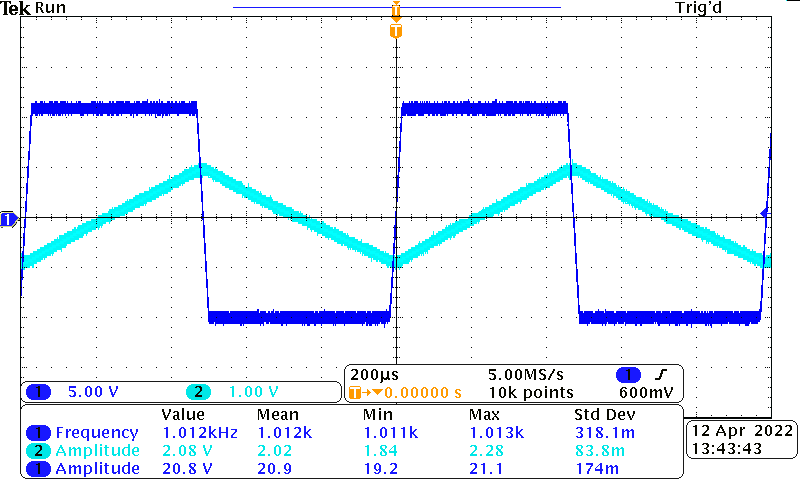
\includegraphics[width=\textwidth]{include/5/1.png}
    \caption{Przebiegi impulsów na wyjściu układu oraz na kondensatorze}
\end{figure}

\begin{figure}[H]
    \centering
    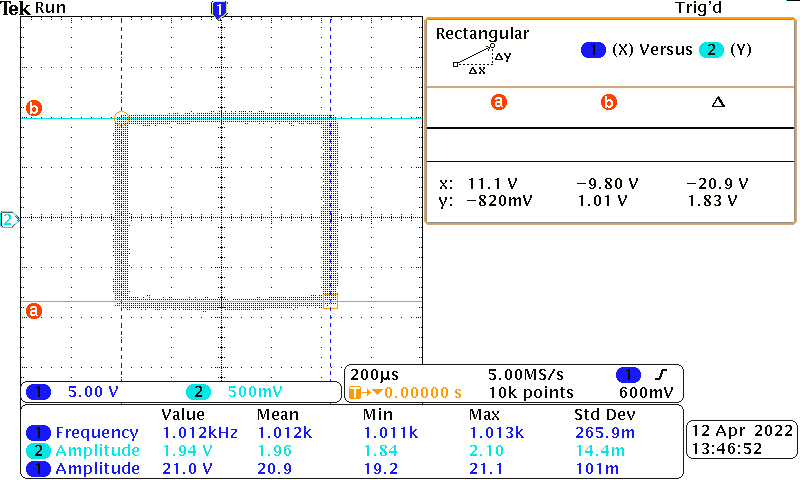
\includegraphics[width=\textwidth]{include/5/2.png}
    \caption{Napięcie na kondensatorze (Y) w funkcji napięcia na wyjściu układu (X)}
\end{figure}
